
%(BEGIN_QUESTION)
% Copyright 2010, Tony R. Kuphaldt, released under the Creative Commons Attribution License (v 1.0)
% This means you may do almost anything with this work of mine, so long as you give me proper credit

Suppose this solenoid control circuit is not working as it should.  When the pushbutton is pressed, the solenoid de-energizes as it should.  However, the solenoid does not {\it remain} de-energized as it should when the pushbutton is released -- instead, it energizes as soon as the switch is released:

$$\includegraphics[width=15.5cm]{i04690x01.eps}$$

A technician has already taken a DC voltage measurement between points C and E with the pushbutton released and the solenoid energized, and measured 0 volts.

\vskip 10pt

Identify the likelihood of each specified fault for this circuit.  Consider each fault one at a time (i.e. no coincidental faults), determining whether or not each fault could independently account for {\it all} measurements and symptoms in this circuit.

% No blank lines allowed between lines of an \halign structure!
% I use comments (%) instead, so that TeX doesn't choke.

$$\vbox{\offinterlineskip
\halign{\strut
\vrule \quad\hfil # \ \hfil & 
\vrule \quad\hfil # \ \hfil & 
\vrule \quad\hfil # \ \hfil \vrule \cr
\noalign{\hrule}
%
% First row
{\bf Fault} & {\bf Possible} & {\bf Impossible} \cr
%
\noalign{\hrule}
%
% Another row
Dead power supply &  &  \cr
%
\noalign{\hrule}
%
% Another row
Relay coil failed open &  &  \cr
%
\noalign{\hrule}
%
% Another row
Pushbutton switch failed open &  &  \cr
%
\noalign{\hrule}
%
% Another row
NO contact failed open &  &  \cr
%
\noalign{\hrule}
%
% Another row
NC contact failed open &  &  \cr
%
\noalign{\hrule}
%
% Another row
Relay coil failed shorted &  &  \cr
%
\noalign{\hrule}
%
% Another row
Pushbutton switch failed shorted &  &  \cr
%
\noalign{\hrule}
%
% Another row
Break in wire between points A and G &  &  \cr
%
\noalign{\hrule}
%
% Another row
Break in wire between points C and E &  &  \cr
%
\noalign{\hrule}
%
% Another row
Break in wire between point F and relay coil &  &  \cr
%
\noalign{\hrule}
} % End of \halign 
}$$ % End of \vbox

\underbar{file i04690}
%(END_QUESTION)





%(BEGIN_ANSWER)

\noindent
{\bf Partial answer:}

\vskip 10pt

% No blank lines allowed between lines of an \halign structure!
% I use comments (%) instead, so that TeX doesn't choke.

$$\vbox{\offinterlineskip
\halign{\strut
\vrule \quad\hfil # \ \hfil & 
\vrule \quad\hfil # \ \hfil & 
\vrule \quad\hfil # \ \hfil \vrule \cr
\noalign{\hrule}
%
% First row
{\bf Fault} & {\bf Possible} & {\bf Impossible} \cr
%
\noalign{\hrule}
%
% Another row
Dead power supply &  & $\surd$ \cr
%
\noalign{\hrule}
%
% Another row
Relay coil failed open &  &  \cr
%
\noalign{\hrule}
%
% Another row
Pushbutton switch failed open &  &  \cr
%
\noalign{\hrule}
%
% Another row
NO contact failed open & &  \cr
%
\noalign{\hrule}
%
% Another row
NC contact failed open &  & $\surd$ \cr
%
\noalign{\hrule}
%
% Another row
Relay coil failed shorted &  &  \cr
%
\noalign{\hrule}
%
% Another row
Pushbutton switch failed shorted &  &  \cr
%
\noalign{\hrule}
%
% Another row
Break in wire between points A and G &  & $\surd$ \cr
%
\noalign{\hrule}
%
% Another row
Break in wire between points C and E &  &  \cr
%
\noalign{\hrule}
%
% Another row
Break in wire between point F and relay coil &  &  \cr
%
\noalign{\hrule}
} % End of \halign 
}$$ % End of \vbox

Many students may find themselves fooled by the 0 volt measurement, thinking this proves points C and E are continuous.  The fallacy at work here is thinking 0 volts proves continuity, just because continuity {\it does} guarantee 0 volts.  In fact, it {\it is} possible for there to be a break between C and E (and still have a 0 volt measurement) if something {\it else} is open within that loop.  For example, the lower NO relay contact could be failed open!

If the same C-to-E measurement were taken with the pushbutton switch pressed, you would find a 24 volt measurement given a broken wire between those two points.

%(END_ANSWER)





%(BEGIN_NOTES)

% No blank lines allowed between lines of an \halign structure!
% I use comments (%) instead, so that TeX doesn't choke.

$$\vbox{\offinterlineskip
\halign{\strut
\vrule \quad\hfil # \ \hfil & 
\vrule \quad\hfil # \ \hfil & 
\vrule \quad\hfil # \ \hfil \vrule \cr
\noalign{\hrule}
%
% First row
{\bf Fault} & {\bf Possible} & {\bf Impossible} \cr
%
\noalign{\hrule}
%
% Another row
Dead power supply &  & $\surd$ \cr
%
\noalign{\hrule}
%
% Another row
Relay coil failed open &  & $\surd$ \cr
%
\noalign{\hrule}
%
% Another row
Pushbutton switch failed open &  & $\surd$ \cr
%
\noalign{\hrule}
%
% Another row
NO contact failed open & $\surd$ &  \cr
%
\noalign{\hrule}
%
% Another row
NC contact failed open &  & $\surd$ \cr
%
\noalign{\hrule}
%
% Another row
Relay coil failed shorted &  & $\surd$ \cr
%
\noalign{\hrule}
%
% Another row
Pushbutton switch failed shorted &  & $\surd$ \cr
%
\noalign{\hrule}
%
% Another row
Break in wire between points A and G &  & $\surd$ \cr
%
\noalign{\hrule}
%
% Another row
Break in wire between points C and E & $\surd$ &  \cr
%
\noalign{\hrule}
%
% Another row
Break in wire between point F and relay coil &  & $\surd$ \cr
%
\noalign{\hrule}
} % End of \halign 
}$$ % End of \vbox















\vskip 20pt \vbox{\hrule \hbox{\strut \vrule{} {\bf Virtual Troubleshooting} \vrule} \hrule}

This question is a good candidate for a ``Virtual Troubleshooting'' exercise.  Presenting the diagram to students, you first imagine in your own mind a particular fault in the system.  Then, you present one or more symptoms of that fault (something noticeable by an operator or other user of the system).  Students then propose various diagnostic tests to perform on this system to identify the nature and location of the fault, as though they were technicians trying to troubleshoot the problem.  Your job is to tell them what the result(s) would be for each of the proposed diagnostic tests, documenting those results where all the students can see.

During and after the exercise, it is good to ask students follow-up questions such as:

\begin{itemize}
\item{} What does the result of the last diagnostic test tell you about the fault?
\item{} Suppose the results of the last diagnostic test were different.  What then would that result tell you about the fault?
\item{} Is the last diagnostic test the best one we could do?
\item{} What would be the ideal order of tests, to diagnose the problem in as few steps as possible?
\end{itemize}


%INDEX% Troubleshooting review: electric circuits

%(END_NOTES)

